\selectlanguage{greek}
\chapter{Πειραματική Διαδικασία}
\label{ch:6.chapterImplementation}

\section{Περιγραφή της πειραματικής διαδικασίας}
Στόχος της πειραματικής διαδικασίας είναι η εφαρμογή των μεθόδων υποβιβασμού τάξης μεγέθους και η χρήση εκτεταμένων υποχώρων \textlatin{Krylov} σε πραγματικά κυκλώματα μεσαίας και μεγάλης κλίμακας. 

Μέσω της τροποποιημένης ανάλυσης κόμβων μετατρέπουμε τα δίκτυα τροφοδοσίας ολοκληρωμένων συστημάτων σε γραμμικά συστήματα στα οποία θα εφαρμόσουμε τον \textlatin{Extended Block Arnoldi (EBA)} αλγόριθμο για να πετύχουμε υποβιβασμό της τάξης μεγέθους και τελικά επίλυση των συστημάτων.

Τα πραγματικά κυκλώματα που θα μελετήσουμε είναι τα δίκτυα τροφοδοσίας των ολοκληρωμένων κυκλωμάτων της ΙΒΜ.

Σαν οδηγό στην υλοποίηση μας χρησιμοποιούμε το εργαλείο \textlatin{MATLAB} το οποίο είναι σχεδιασμένο για γρήγορη και άμεση υλοποίηση (χρησιμοποιώντας συναρτήσεις συστήματος για τις περισσότερες πράξεις μεταξύ πινάκων) αλγορίθμων.

Με τη βοήθεια του παραπάνω εργαλείου μπορούμε να αξιοποιήσουμε ότι η υλοποίηση μας είναι ορθή σε όλα τα στάδια της.

\subsection{Μορφή αρχείων εισόδου}
Τα αρχεία εισόδου είναι σε μορφή \textlatin{Matrix Market}. Περιγραφή της παραπάνω μορφής μπορείτε να βρείτε στο Παράρτημα \ref{ch:chapterMatrixMarketFormat}. Όπως μπορούμε να παρατηρήσουμε στη μορφή του αρχείου, ο πίνακας ξκινάει απο τη θέση 1,1. Στις δομές δεδομένων που χρησιμοποιούμε (όπως είναι η Τρίδυμη Δομή Απεικόνισης \ref{TripletForm} και Δομή της Συμπιεσμένης Στήλης \ref{CCS}) στην υλοποίηση μας, οι πίνακες έχουν σαν αρχικές συντεταγμένες το $(0,0)$. Συνεπώς, μια βασική αλλαγή που πρέπει να πραγματοποιήσουμε είναι να αφαιρούμε -1 από κάθε συντεταγμένη γραμμής και στήλης έτσι ώστε να έχουμε τον ίδιο πίνακα.

\subsection{Επέκταση υπάρχουσας βιβλιοθήκης \textlatin{CSparse}}

Η βιβλιοθήκη \textlatin{CSparse} που χρησιμοποιήσαμε κατά την υλοποίηση μας περιλαμβάνει ένα πλήθος συναρτήσεων για πράξεις για διαχείριση και πραγματοποίηση πράξεων μεταξύ αραιών πινάκων (Παράρτημα \ref{ch:chapterCSparse}). Για την υλοποίηση του αλγορίθμου \textlatin{EBA} (Κεφάλαιο \ref{EBA}) χρειάστηκε να υλοποιήσουμε επιπλέον συναρτήσεις τις πιο σημαντικές από τις οποίες θα αναφέρουμε στη συνέχεια.

\subsection{Ανάκτηση πίνακα $Q$ απο τα διανύσματα \textlatin{Householder}}

Η βιβλιοθήκη \textlatin{CSparse} κατά την παραγοντοποίηση $QR$ χρησιμοποιεί τη μέθοδο \textlatin{Householder} (Κεφάλαιο \ref{HouseholderMethod}). Η μέθοδος αυτή αν και εξαιρετικά αποτελεσματική για επίλυση προβλημάτων όπως των Ελαχίστων Τετραγώνων, στη δική μας περίπτωση όπου χρειαζόμαστε τον άνω τριγωνικό πίνακα $Q$, τα διανύσματα απεικόνισης (\textlatin{reflectors}) δεν μπορούν να χρησιμοποιηθούν στην επίλυση μας. Συνεπώς, θα χρειαστεί να πραγματοποιήσουμε ένα επιπλέον βήμα όπου απο τα διανύσματα απεικόνισης (\textlatin{reflectors}) θα χρειαστεί να ανακτήσουμε τον πίνακα $Q$.

\subsubsection{Μέθοδοι Ανάκτησης Πίνακα Παραγόντων $Q$}

Στις περιπτώσεις όπου χρειάζεται η ανάκτηση του πίνακα παραγόντων $Q$ μπορούμε να ακολουθήσουμε τις παρακάτω μεθόδους ~\cite{van1983matrix}:
\begin{itemize}
    \item \textbf{Εμπρόσθια Συσσώρευση} (\textlatin{Forward Accumulation})
    Για την ανάκτηση του πίνακα $Q$ με την παραπάνω μέθοδο ακολουθούμε τον εξής αλγόριθμο:\\\\
    \selectlanguage{english}
    \begin{algorithm}[H]
        \SetAlgoLined
        \caption{\selectlanguage{greek} Εμπρόσθια Συσσώρευση(\textlatin{Forward Accumulation})}
        $Q = I_n$\\
        \For{$j\gets1$ \KwTo $r$ \KwBy $1$}{
            $Q = Q Q_j$
        }
    \end{algorithm}
    \selectlanguage{greek}
    \item \textbf{Οπίσθια Συσσώρευση} (\textlatin{Backward Accumulation})\\
    \selectlanguage{english}
    \begin{algorithm}[H]
        \SetAlgoLined
        \caption{\selectlanguage{greek} Οπίσθια Συσσώρευση(\selectlanguage{english}Backwards Accumulation\selectlanguage{greek})}
        $Q = I_n$\\
        \For{$j\gets r$ \KwTo $1$ \KwBy $-1$}{
            $Q = Q_j Q$
        }
    \end{algorithm}
    \selectlanguage{greek}
    
    Μπορεί εύκολα να αποδειχθεί ότι το $(j-1)x(j-1)$ κομμάτι του $Q_j$ είναι ο ταυτοτικός πίνακας όποτε κατά το ξεκίνημα της Οπίσθιας Συσσώρευσης, ο $Q$ κατά κύριο λόγο είναι ο ταυτοτικός πίνακας και σε κάθε βήμα γίνεται όλο και πιο πλήρης όσο ο αλγόριθμος εξελίσσεται. Το συγκεκριμένο χαρακτηριστικό του αλγορίθμου μπορεί να αξιοποιηθεί έτσι ώστε να μειώσουμε τον αριθμό των πράξεων που χρειάζονται. Σε αντίθεση, στην Εμπρόσθια Συσσώρευση, μετά το πρώτο βήμα, ο πίνακας είναι ήδη πλήρης. Με βάση τα παραπάνω, ο αλγόριθμος μπορεί να μετατραπεί:\\
    
    \selectlanguage{english}
    \begin{algorithm}[H]
        \SetAlgoLined
        \caption{\selectlanguage{greek} Βελτιωμένη Οπίσθια Συσσώρευση(\selectlanguage{english}Backwards Accumulation\selectlanguage{greek})}
        $Q = I_n$\\
        \For{$j\gets r$ \KwTo $1$ \KwBy $-1$}{
            $v(j:n) = $\begin{bmatrix}
                        1 \\
                        A(j+1:n,j)
                        \end{bmatrix}\\
            $Q(j:n,j:n) = (I - \beta_j v(j:n) v(j:n)^T) Q(j:n,j:n)$
        }
    \end{algorithm}
\end{itemize}

Στα πλαίσια της διπλωματικής εργασίας, εφαρμόσαμε τον αλγόριθμο Βελιτωμένης Οπίσθιας Συσσώρευσης.

\section{Αποτελέσματα Πειραματικής Διαδικασίας}

Για την αξιολόγηση της πειραματικής διαδικασίας διαλέξαμε τα διαθέσιμα πλέγματα ενέργειας \textlatin{power grids} της \textlatin{IBM} ~\cite{nassif2008power}. Τα χαρακτηριστικά των παραπάνω πλεγμάτων ενέργειας μπορούν να συνοψιστούν στον παρακάτω πίνακα \ref{table:1}:

\begin{table}[h!]
\centering
 \begin{tabular}{||c | c | c||} 
 \hline
 Αρχείο Εισόδου & Διαστάσεις & \textlatin{\#}είσοδων \\ [0.5ex] 
 \hline\hline
 \textlatin{ibmpg1} & 44946 & 600 \\ 
 \hline
 \textlatin{ibmpg2} & 127568 & 500 \\
 \hline
 \textlatin{ibmpg3} & 852539 & 800 \\
 \hline
 \textlatin{ibmpg4} & 954545 & 600 \\
 \hline
 \textlatin{ibmpg5} & 1618397 & 600 \\
 \hline
 \textlatin{ibmpg6} & 2506733 & 1000 \\
 \hline
 \textlatin{ibmpg1t} & 54265 & 400 \\
 \hline
 \textlatin{ibmpg2t} & 164897 & 800 \\
 \hline
\end{tabular}
\caption{Πίνακας περιγραφής διαστάσεων και \textlatin{\#}εισόδων για τα πλέγματα ενέργειας \textlatin{IBM}}
\label{table:1}
\end{table}

\subsection{Απαραίτητες τροποποιήσεις πλεγμάτων ενέργειας}
Στον παραπάνω πίνακα \ref{table:1} παρατηρούμε στις 2 τελευταίες γραμμές τα πλέγματα ενέργειας \textlatin{ibmpg1t, ibmpg2t}. Τα 2 αυτά πλέγματα ενέργειας έχουν το γράμμα \textlatin{t} στο τέλος το οποίο υποδηλώνει οτι αναφέρονται στην μεταβατική \textlatin{transient} ανάλυση. Τα πλέγματα ενέργειας που αναφέρονται στην μεταβατική ανάλυση, χρειάζεται να παρέχουμε έναν πίνακα με στοιχεία αποθήκευσης ενέργειας (πυκνωτές και πηνία). Από την άλλη μεριά, για να πραγματοποιήσουμε μεταβατική ανάλυση στα πλέγματα ενέργειας συνεχούς \textlatin{DC} ροής, στην προκειμένη περίπτωση \textlatin{ibmpg1 - ibmpg6} έπρεπε να προσθέσουμε έναν διαγώνιο πίνακα με πυκνωτικά στοιχεία τα οποία είχαν τυχαίες τιμές της τάξης του \textlatin{picofarad}. Η παραπάνω προσθήκη είναι τυπική για τέτοιου είδους πλέγματα ενέργειας.


\subsection{Αξιολόγηση πλεγμάτων ενέργειας αναφοράς}
Για να καταφέρουμε να αξιολογήσουμε την μεθοδολογία μας σε μοναδικά πλέγματα ενέργειας αναφοράς, επιβάλαμε στον πίνακα πυκνωτικών στοιχείων των πλεγμάτων \textlatin{ibmpg2} και \textlatin{ibmpg4} να έχουν τουλάχιστον έναν κόμβο ο οποίος δεν είχε ένωση με πυκνωτικό στοιχείο. Τα παραπάνω πλέγματα αναφοράς καθώς μαζί με τα \textlatin{ibmpg1t} και \textlatin{ibmpg2t} αντιπροσωπεύονται ως μοναδικά μοντέλα περιγραφής του ~\cite{nassif2008power}. %εφαρμόσαμε τις μεθόδους που περιγράφονται στο ΙΙΙ-Β


\subsection{Εφαρμογή και σύγκριση με υπάρχουσες μεθόδους}
Όπως έχουμε τονίσει και σε προηγούμενα κεφάλαια, στα πλαίσια της διπλωματικής εργασίας, εφαρμόσαμε τον αλγόριθμο \textlatin{Extended Block Arnoldi (EBA)} τον οποίο περιγράψαμε στο \ref{EBA} και τον συγκρίναμε με μια βασική υλοποίηση Αντιστοίχισης Στιγμών (\textlatin{Moment-Matching (MM)} η οποία επίσης χρησιμοποιούσε την αρχή της επαλληλίας(\textlatin{superposition property}). Τα μοντέλα μειωμένης τάξης (\textlatin{Reduced-Order Models (ROMs)}) αξιολογήθηκαν στο εύρος συχνοτήτων $[10^0, 10^{12}]$ συναρτήσει της ακρίβειας για τη δεδομένη τάξη του μοντέλου.

Για την αξιολόγηση μας επιλέξαμε τον κατάλληλο αριθμό στιγμών για το κάθε πλέγμα ενέργειας έτσι ώστε και η μέθοδος \textlatin{EBA} που εφαρμόσαμε αλλά και η κλασσική \textlatin{MM} μέθοδος να καταλήγουν στην ίδια τάξη μοντέλου.


\subsection{Πίνακες συνολικών αποτελεσμάτων και περιγραφή μεταβλητών σύγκρισης}

Στη συνέχεια παραθέτουμε πίνακες με τα αποτελέσματα της ανάλυσης μας. Οι πίνακες περιλαμβάνουν τα δεδομένα για την εκτέλλεση της βασικής μεθόδου Αντιστοίχισης Στιγμών (\textlatin{Moment-Matching (MM)}, της εκτέλεσης της μεθόδου Εκτεταμένου Υποχώρου \textlatin{Krylov} (\textlatin{EBA}) καθώς και έναν πίνακα με τη σύγκριση των λαθών για κάθε πλέγμα ενέργειας.

Ξεκινάμε παραθέτωντας τα αποτελέσματα κατα την εφαρμογή της βασικής μεθόδου Αντιστοίχισης Στιγμών (\textlatin{Moment-Matching (MM)} ~\ref{table:BasicMM}.

\begin{table}[h!]
\centering
 \begin{tabular}{||c | c | c||} 
 \hline
 Αρχείο Εισόδου & \textlatin{\#}στιγμών & Μέγιστο Λάθος \\ [0.5ex] 
 \hline\hline
 \textlatin{ibmpg1} & 2 & 0.037 \\ 
 \hline
 \textlatin{ibmpg2} & 4 & 0.233 \\
 \hline
 \textlatin{ibmpg3} & 2 & 0.253 \\
 \hline
 \textlatin{ibmpg4} & 4 & 0.233 \\
 \hline
 \textlatin{ibmpg5} & 2 & 0.242 \\
 \hline
 \textlatin{ibmpg6} & 6 & 0.161 \\
 \hline
 \textlatin{ibmpg1t} & 2 & 4.767 \\
 \hline
 \textlatin{ibmpg2t} & 4 & 0.785 \\
 \hline
\end{tabular}
\caption{Πίνακας αποτελεσμάτων του μέγιστου λάθους με την εφαρμογή βασικής μεθόδου Αντιστοίχισης Στιγμών για τα πλέγματα ενέργειας \textlatin{IBM}}
\label{table:BasicMM}
\end{table}



Συνεχίζουμε παραθέτοντας τα αποτελέσματα κατά την εφαρμογή της μεθόδου Εκτεταμένου Υποχώρου \textlatin{Krylov} (\textlatin{EBA}) ~\ref{table:ResultsEBAMaxError}.

\begin{table}[h!]
\centering
 \begin{tabular}{||c | c | c||} 
 \hline
 Αρχείο Εισόδου & \textlatin{\#}στιγμών & Μέγιστο Λάθος \\ [0.5ex] 
 \hline\hline
 \textlatin{ibmpg1} & 1 & 0.014 \\ 
 \hline
 \textlatin{ibmpg2} & 2 & 0.131 \\
 \hline
 \textlatin{ibmpg3} & 1 & 0.146 \\
 \hline
 \textlatin{ibmpg4} & 2 & 0.038 \\
 \hline
 \textlatin{ibmpg5} & 1 & 0.063 \\
 \hline
 \textlatin{ibmpg6} & 3 & 0.130 \\
 \hline
 \textlatin{ibmpg1t} & 1 & 1.814 \\
 \hline
 \textlatin{ibmpg2t} & 2 & 0.411 \\
 \hline
\end{tabular}
\caption{Πίνακας αποτελεσμάτων του μέγιστου λάθους με την εφαρμογή μεθόδου Εκτεταμένου Υποχώρου \textlatin{Krylov} (\textlatin{EBA}) για τα πλέγματα ενέργειας \textlatin{IBM}}
\label{table:ResultsEBAMaxError}
\end{table}

Τέλος παραθέτουμε τα αποτελέσματα της σύγκρισης μεταξύ των 2 παραπάνω μεθόδων και το ποσοστό μείωσης λάθους της μεθόδου Εκτεταμένου Υποχώρου \textlatin{Krylov} (\textlatin{EBA}) σε σχέση με τη βασική μέθοδο ~\ref{table:ResultsEBAMaxErrorCompared}:

\begin{table}[h!]
\centering
 \begin{tabular}{||c | c | c | c||} 
 \hline
 Αρχείο Εισόδου & Μέγιστο Λάθος (\textlatin{MM}) & Μέγιστο Λάθος \textlatin{EKS(EBA)-MM} & Ποσοστό Μείωσης Λάθους \\ [0.5ex] 
 \hline\hline
 \textlatin{ibmpg1} & 0.037  & 0.014 & 62.16\% \\ 
 \hline
 \textlatin{ibmpg2} & 0.233 & 0.131 & 43.78\% \\
 \hline
 \textlatin{ibmpg3} & 0.253 & 0.146 & 42.29\% \\
 \hline
 \textlatin{ibmpg4} & 0.233 & 0.038 & 83.69\% \\
 \hline
 \textlatin{ibmpg5} & 0.242 & 0.063 & 73.97\% \\
 \hline
 \textlatin{ibmpg6} & 0.161 & 0.130 & 19.25\% \\
 \hline
 \textlatin{ibmpg1t} & 4.767 &  1.814 & 61.95\% \\
 \hline
 \textlatin{ibmpg2t} & 0.785 &  0.411 & 47.64\% \\
 \hline
\end{tabular}
\caption{Πίνακας αποτελεσμάτων σύγκρισης του μέγιστου λάθους μεταξύ των μεθόδων για τα πλέγματα ενέργειας \textlatin{IBM}}
\label{table:ResultsEBAMaxErrorCompared}
\end{table}

Για τους πίνακες ~\ref{table:ResultsEBAMaxError},~\ref{table:ResultsEBAMaxErrorCompared} το Μέγιστο Λάθος αναφέρεται στο λάθος μεταξύ των άπειρων νορμών των συναρτήσεων μεταφοράς. Στην προκειμένη περίπτωση, για τα αρχεία εισόδου έχουμε $|| \Tilde{H(s) - H(s)||_\infty}$


Βλέπουμε επίσης στον πίνακα ~\ref{table:ResultsEBAMaxErrorCompared} οτι η ποσοστιαία μείωση του λάθους κυμαίνεται από $19.25\%$ έως $83.69\%$.

Για την καλύτερη απεικόνιση των αποτελεσμάτων, επιλέξαμε να δείξουμε ενδεικτικά τις συναρτήσεις μεταφοράς για τις δύο μεθόδους που υλοποιήσαμε (\textlatin{EKS-MM, MM}) με αρχεία εισόδου \textlatin{ibmpg1, ibmpg2t, ibmpg6} καθώς και το μέγεθος λάθους με αρχείο εισόδου \textlatin{ibmpg6}. Σαν σημείο αναφοράς έχουμε συμπεριλάβει και την αρχική συνάρτηση μεταφοράς.


\begin{figure}[h!]
\caption{Σύγκριση της συνάρτηση μεταφοράς στα υποβιβασμένης τάξης μοντέλα (\textlatin{Reduced Order Models (ROMs)} με τη χρήση της μεθόδου \textlatin{EKS-MM} και της κλασσικής μεθόδου \textlatin{MM} στο εύρος συχνοτήτων $[10^0, 10^{12}]$ για το αρχείο εισόδου \textlatin{ibmpg1} για θύρες (9,9)}
\centering
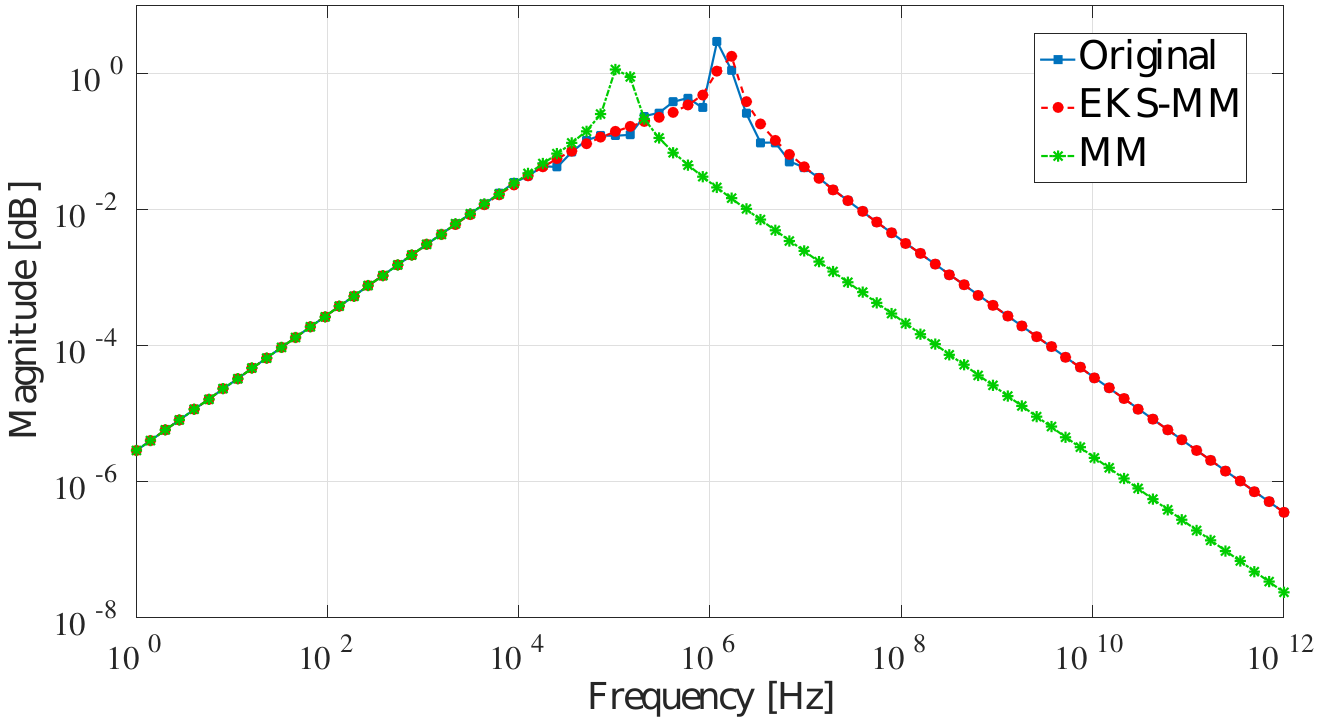
\includegraphics[width=\textwidth,height=\textheight,keepaspectratio]{FrequencyResponseAtPort9_9ofIbmpg1}
\end{figure}



\begin{figure}[h!]
\caption{Σύγκριση της συνάρτηση μεταφοράς στα υποβιβασμένης τάξης μοντέλα (\textlatin{Reduced Order Models (ROMs)} με τη χρήση της μεθόδου \textlatin{EKS-MM} και της κλασσικής μεθόδου \textlatin{MM} στο εύρος συχνοτήτων $[10^0, 10^{12}]$ για το αρχείο εισόδου \textlatin{ibmpg2t} για θύρες (4,4)}
\centering
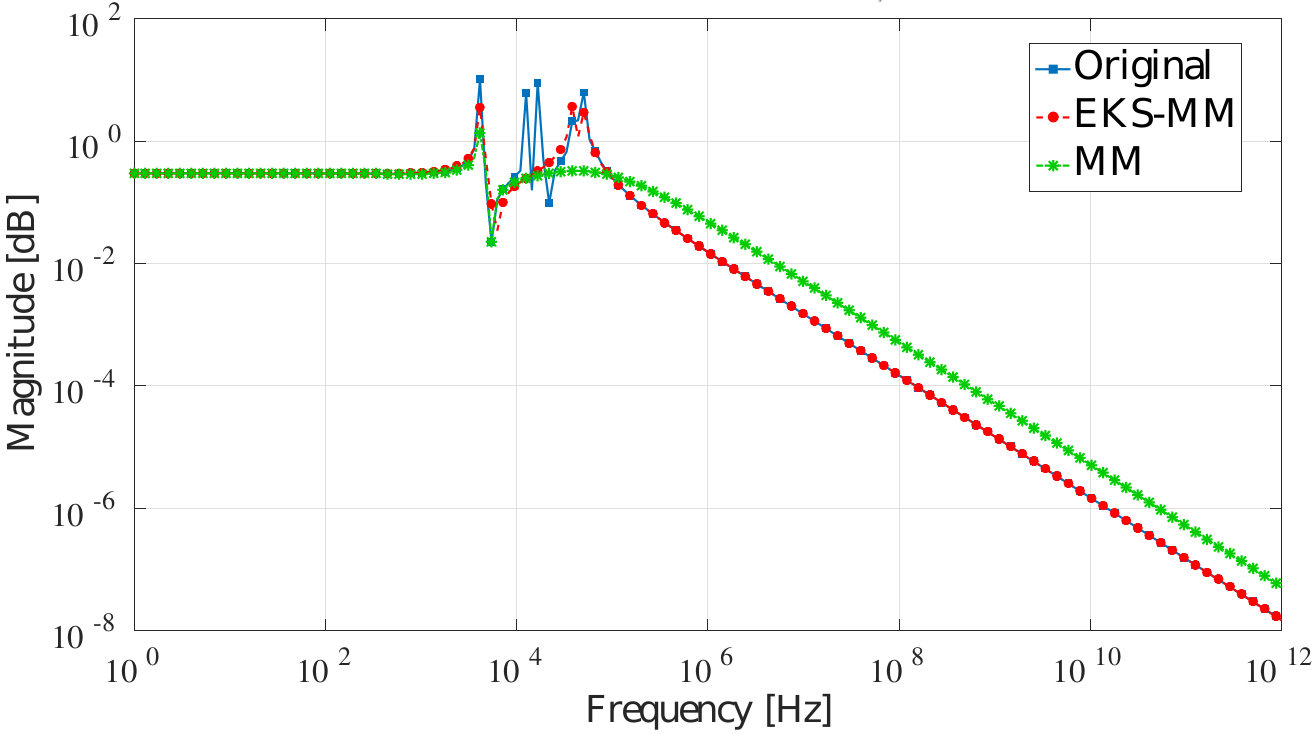
\includegraphics[width=\textwidth,height=\textheight,keepaspectratio]{FrequencyResponseAtPort4_4Ibmpg2t}
\end{figure}

\begin{figure}[h!]
\caption{Σύγκριση της συνάρτηση μεταφοράς στα υποβιβασμένης τάξης μοντέλα (\textlatin{Reduced Order Models (ROMs)} με τη χρήση της μεθόδου \textlatin{EKS-MM} και της κλασσικής μεθόδου \textlatin{MM} στο εύρος συχνοτήτων $[10^0, 10^{12}]$ για το αρχείο εισόδου \textlatin{ibmpg6} για θύρες (5,5)}
\centering
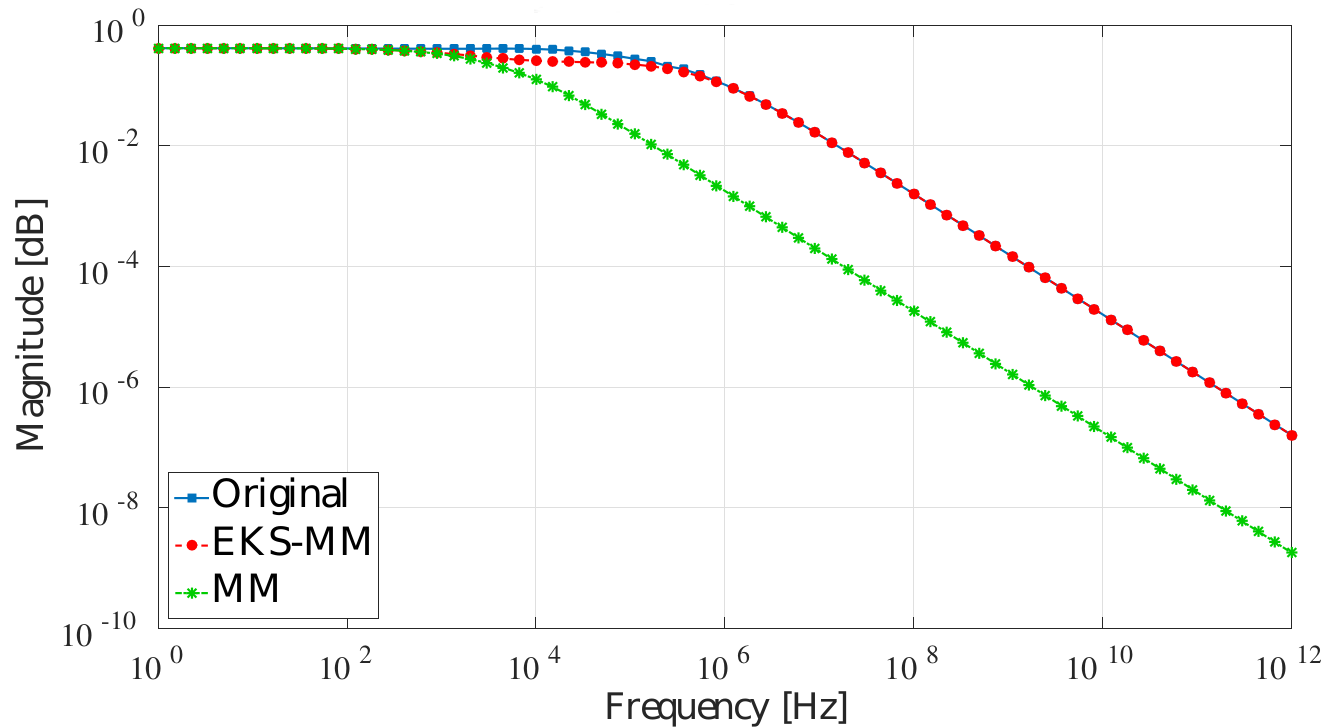
\includegraphics[width=\textwidth,height=\textheight,keepaspectratio]{FrequencyResponseAtPort5_5Ibmpg6}
\end{figure}

\begin{figure}[h!]
\caption{Μέγεθος του λάθους για τα υποβιβασμένης τάξης μοντέλα (\textlatin{Reduced Order Models (ROMs)} με τη χρήση της μεθόδου \textlatin{EKS-MM} και της κλασσικής μεθόδου \textlatin{MM} στο εύρος συχνοτήτων $[10^0, 10^{12}]$ για το αρχείο εισόδου \textlatin{ibmpg6} για θύρες (5,5)}
\centering
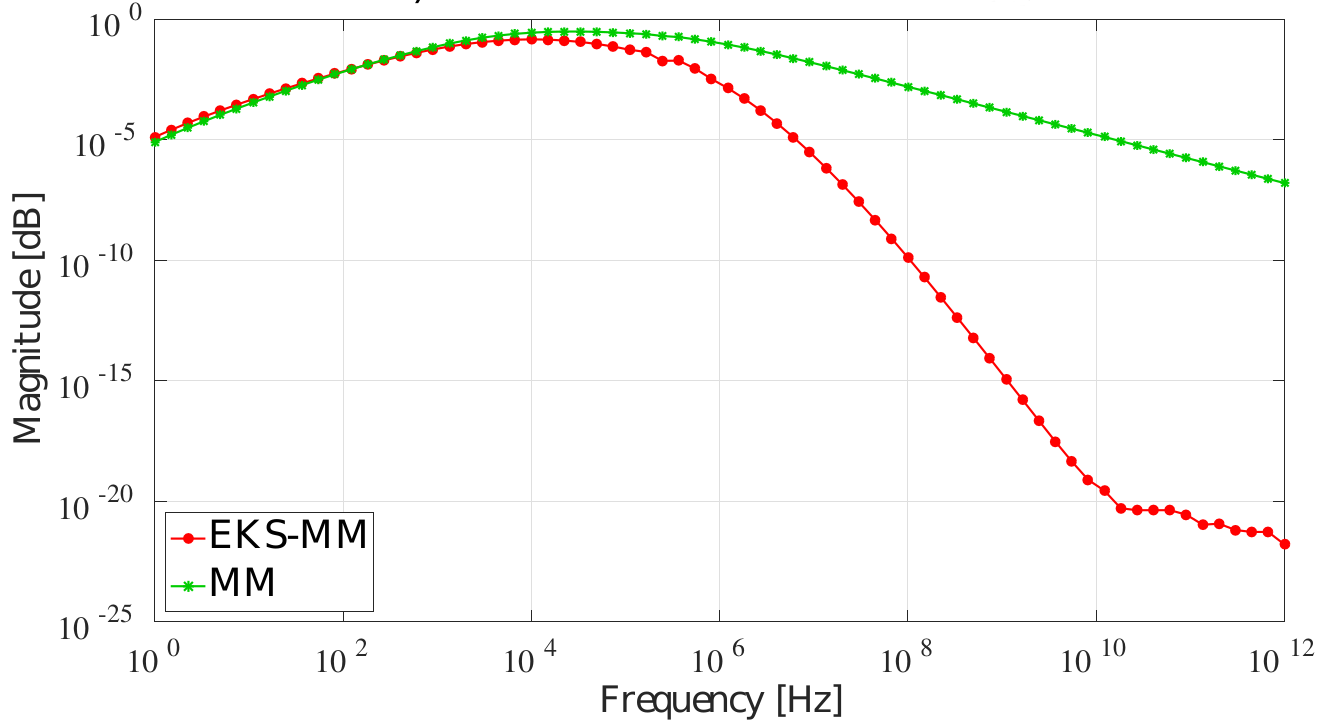
\includegraphics[width=\textwidth,height=\textheight,keepaspectratio]{MORErrorAtPort5_5Ibmpg6}
\end{figure}
